% Chapter 2

\chapter{Hardware} % Main chapter title

\label{Chapter2} % For referencing the chapter elsewhere, use \ref{Chapter1} 

\lhead{Chapter 2. \emph{Hardware}} % This is for the header on each page - perhaps a shortened title

%----------------------------------------------------------------------------------------

\section{Hardware}

\subsection{Inverter System Overview}

The inverter is responsible for converting the DC power output by the photovoltaic panels into the 120Vrms power used by the power grid. The heart of the inverter is the C2000 microcontroller by Texas Instruments which implements the Hybrid control algorithm for power switching. The microinverter has three main power conversion stages: boost converter, inverter, and output filter. The boost converter increases low panel voltage up to 200V while implementing maximum power point tracking for the PV panel. The inverter consists of an H-Bridge that creates the AC wave with 169.73V peak voltage. The output filter removes high frequency switching noise and passes the 60Hz intended for standard loads.  Feedback control operation requires voltages and currents to be measured in real time by the microcontroller analog-to-digital converter. Logic and signal conditioning power is sourced through an auxiliary power supply which steps down solar input voltage. This system is represented in the depiction found in Figure~\ref{Figure 1}.   

\subsection{Logic Power Supply}
A logic power supply was required for the inverter board to run the microcontroller, driver circuits, peripheral sensor network. Three different voltage rails were needed at 12V, 5V and 3.3V. The input from the solar panel was utilized to create these different power rails through a small connection circuit. Efficiency of this type of system is considered crucial, so cascaded switching DC/DC buck converters were used to create the 12V and 5V rails. A fast responding low-dropout linear regulator created the final 3.3V from the 5V rail. The circuit schematic for the logic power supply is shown in Figure~\ref{logic power fig}.

A variety of features were added to this front input interface for system protection and functionality. There are two options for sourcing power to the inverter board: banana jack connections for solar input and a DC barrel jack plug for testing input. These two circuits are configured so that only the barrel jack will source power if both happened connected and energized at the same time. Two switches are included for toggling the DC jack input and for switching conversion power into the main system. A ten amp blow fuse is included in series with the input to the inverter to prevent damaging short circuit conditions. A green LED on the 3.3V rail turns on to show the system is properly functioning.

\subsection{Boost Converter}
A standard PV microinverter contains two principle energy conversion stages with a DC/DC module and DC/AC module. This section highlights the design process of a DC/DC boost converter for solar microinverter implementations. The boost circuit includes many elements and considerations of the final inverter system including power switching hardware and sensor circuits.

The boost stage designed is essential for photovoltaics since it allows consistent maximum power sourcing from the panel. Solar panels have nonlinear relationships between output voltage and current. The maximum power product of the electrical values will vary depending on light intensity levels, loading, and temperature. A microcontroller unit (MCU) is used with this boost converter for create a feedback control scheme called a maximum power point tracker (MPPT). A versatile DC/DC boost stage is needed for microinverters since it can dynamically vary power switching based on the MPPT to compensate for the wide range of potential solar panel voltages. This converter topology utilizes a discrete MOSFET for switching since microcontroller interfacing is required. Traditional boost converter integrated circuits (ICs) do not satisfy the MPPT control needs or power requirements needed for this type of system.  


A generic boost converter circuit shown in Figure~\ref{Figure 3}. Operation of a boost converter has two distinct phases depending on the switch mode of the power MOSFET. The gate of the MOSFET is sent different logic values at specific duty cycles through PWM. When the drive circuit outputs logic high in Figure 3, the drain to source path will conduct in the saturation region. This provides a path to ground for the current flowing through the inductor and reverse biases the clamp diode. Over time energy is built up in the magnetic field of the inductor coil from this solar panel sourced current. Then logic low is sent to the MOSFET to shut it down. Considering the sudden change in current flow, a large voltage kickback occurs across the inductor and forward biases the diode. Current now can flow to charge the output capacitor and feed the load.

\begin{figure}
\centering
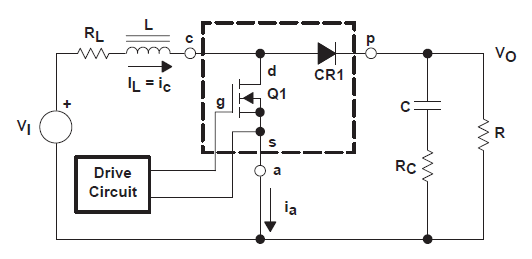
\includegraphics[width = 3.5in]{Generic_Boost_Converter.PNG}
\caption{Traditional Boost Converter Circuit}
\label{Figure 3}
\end{figure}


When the MOSFET is conducting, the output capacitor provides power to the load until it receives new charge during the second period. Due to the switching characteristics and inductor physics, a large ripple current flows through the inductor. An important design constraint it to make sure the inductor current always remains greater than zero such that continuous conduction mode (CCM) is maintained. CCM ensures a desired voltage transfer function for gain in this design. Additionally, there are some parasitic elements included in the circuit that contribute to power loss. These undesired effects include the DC resistance of the inductor windings and the equivalent series resistance of the capacitor.  
The electrical specifications of this boost converter are listed in Table~\ref{Table 1}. \\ 


\begin{table}
\centering
\begin{tabular}{|c|c|}
\hline
 Parameter & Value \\
 \hline
 $ V_{in} = V_{panel}$ & 0V to 40V DC \\
 \hline
 $ I_{in}$ & 5.47A DC max \\
 \hline
 $ V_{out}=V_{load} $ & 169.73V Min to 200V max \\
 \hline
 $ I_{out} $ & 1.18A DC max \\
 \hline
 $ P_{rated} $ & 200W \\
 \hline
 $ f_{switching} $ & 50 kHz \\
 \hline
\end{tabular}
\caption{Electrical Specifications for Boost Converter}
\label{Table 1}
\end{table}

The Sharp solar panels, utilized in this design as an input power source, will have varying voltage and current output capabilities depending on lighting conditions. Maximum output power for the 170W panels occurs at $V_{panel}=34.8V$ and  $I_{panel} = 4.9A$. A input voltage range will be selected to define a sourcing range with usable power output considering the panels highly nonlinear relationship regarding I vs V shown in Figure~\ref{Figure 4}. Output voltage is defined based on the minimum value needed for the 120Vrms/0.707 = 169.73V peak value needed for the DC/AC inverter stage input. Maximum power of 200W is an upper limit buffer set for this design considering the solar panel approach with microinverter topology. Switching frequency is set at 50 kHz based on recommended ranges and to compare to the TI Solar Explorer Development Board also used in this project.\cite{SharpPanel}

\begin{figure}
\centering
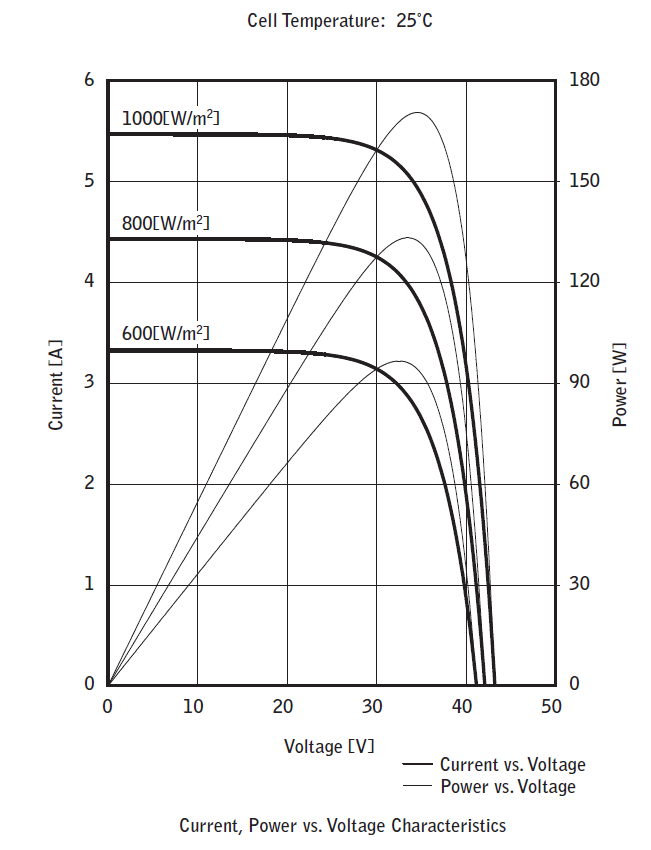
\includegraphics[width = 3.5in]{solar_v_vs_i.PNG}
\caption{Solar Panel IV Characteristics}
\label{Figure 4}
\end{figure}

The process of designing the boost circuit hardware involved research of reference application notes and in running PSPICE simulations. PSPICE computer software produced by Cadence\textbackslash{}OrCAD was used to simulate the boost converter circuit. The max power voltage of the PV panels was selected for primary simulation testing. Calculations were performed to best select power components for operations of the boost converter at high power values. These design steps considered power dissipation thermal limits, critical inductance, and critical capacitance. The PSPICE circuit encapsulating the entire boost converter design is shown in Figure~\ref{boostCrct}.

\begin{figure}
\centering
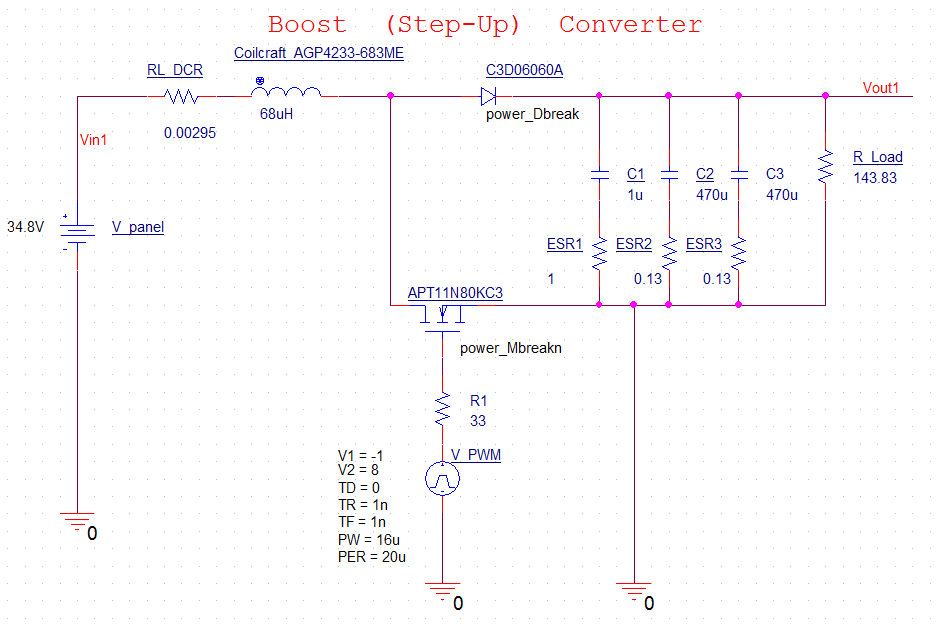
\includegraphics[width = 3.5in]{Boost_Circuit.PNG}
\caption{PSPICE Boost Converter Simulation}
\label{boostCrct}
\end{figure}

The operation of the boost converter in PSPICE required a switching signal to control the power MOSFET. Implementation of the converter will utilize C2000 MCU logic signals and Silicon Labs gate driver circuits for MOSFET switching. This simulation uses a variable duty cycle pulse source for continuous switching at the set frequency. This configuration is currently being run open-loop, but will include a compensation feedback control circuit to maintain stable output voltage in the final design. The solar panel 34.8V input at max power required a duty cycle set at 80.13\% for the PWM switching signal to achieve 169.73Vdc out. A load of 143.83$\Omega$ was connected at the output to simulate max power current draw and realize the 200W capability of the system. Real output power will be less in practice due to additional inefficiencies, panel operating conditions, and sourcing configuration capabilities. The output power, current and voltage as the boost converter approaching steady-state conditions from start-up are shown in the simulation plot of Figure~\ref{Figure B}.

\begin{figure}
\centering
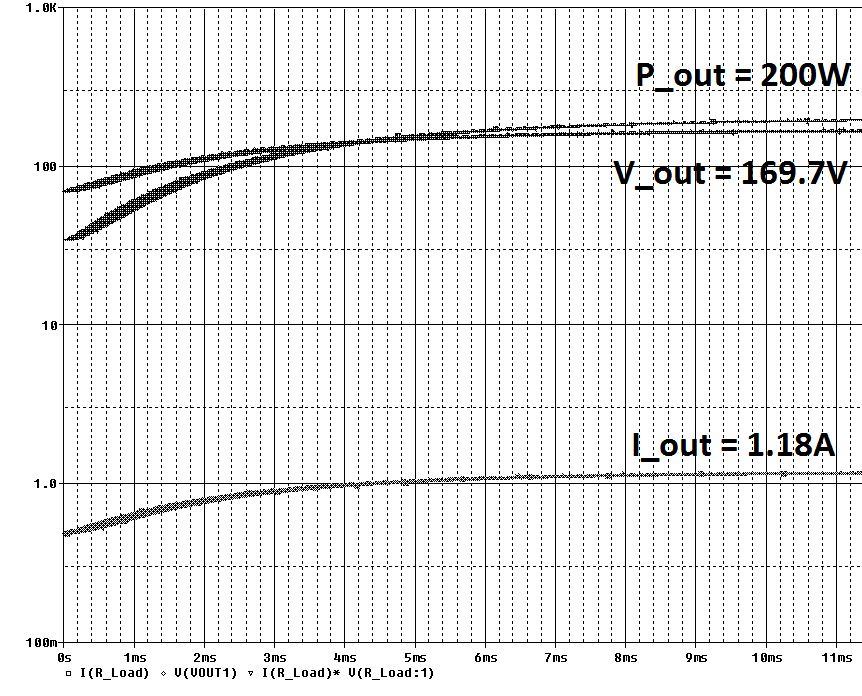
\includegraphics[width = 3.5in]{Boost_Power.png}
\caption{Boost Converter Approaching Steady State}
\label{Figure B}
\end{figure}

This boost converter was designed to operate in continuous condition mode (CCM). Ensuring this condition meant that the inductor current will never fall to zero and the panels are always sourcing current. This was achieved by selecting an inductor value above the calculated critical inductance and making sure it has appropriate current handling capabilities. Figure~\ref{Figure c} shows the rippled inductor current in CCM and the MOSFET switching signal that creates these dynamic effects in the boost converter. 

\begin{figure}
\centering
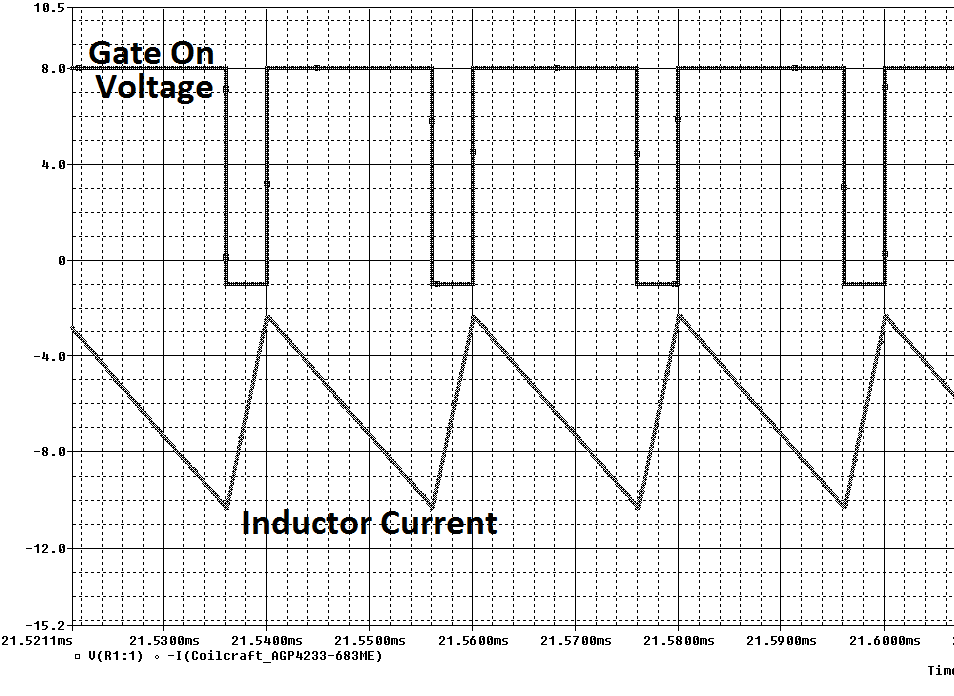
\includegraphics[width = 3.5in]{Boost_Inductor_Current_Steady_State.png}
\caption{Switching Signal and Inductor Current}
\label{Figure c}
\end{figure}

Another factor that will influence the switching of the MOSFET is the maximum power-point tracking (MPPT) algorithm implemented by the microcontroller. This works to vary the input impedance of the converter as seen by the panel to optimize power output at 34.8V. This method uses feedback control based on the voltage and currents measured by the ADC to perturb and observe the boost condition. Since the solar panel voltage can vary, the simulation circuit was run at the minimum 20V to check that the power output voltage could be maintained. The simulation results confirm this with $V_{out}=169.73V$, $V_{panel,in}=20V$, and a new duty cycle set at 89.25\%.

Ratings on voltages and currents concerning components were determined through worst case calculations.\cite{kwasinski} 
\begin{equation}
I_L = I_{diode} = I_{drain} = \frac{2}{\sqrt[2]{3}}I_{in,rms} 
\end{equation}
\begin{equation}
 V_{cap} = V_{out} = 1.5V_{out,typ} = 2(169.73V) = 254.6V 
\end{equation}
\begin{equation}
 V_{diode} = V_{DS,FET} = 2(169.73V) =339.46V  
\end{equation}
\begin{equation}
I_{cap} = I_{out,rms} = 1.18A 
\end{equation}
The clamp diode was selected to be a SiC schottky type since it offers fast recovery times with low reverse recovery charge $Q_{rr}$ for reduced switching losses. Since the diode resides in the power conduction path, energy dissipation was analyzed. The diode was modeled as a series circuit of a temperature dependent voltage source $ V_{diode}$ and resistance $R_{diode}$.\cite{CREE}
\begin{equation}
 V_{diode} = \alpha T_{junction}+V_{diode,0} =  0.95V 
\end{equation}
\begin{equation}
 R_{diode} = \beta T_{junction}+R_{diode,0} = 0.103\Omega
\end{equation}
\begin{equation}
 P_{cond} = {I_{diode,rms}}^2R_{diode}+I_{out,max}V_{diode} = 2.76W
\end{equation}
\begin{equation}
 I_{diode,rms} = \frac{I_{out}}{\eta} \sqrt[2]{ \frac{16V_{out}}{3 \pi V_{in}}}= 3.99A
\end{equation}
\begin{equation}
P_{switching} = Q_{c,diode}V_{out}f_{sw}=0.14W
\end{equation}
\begin{equation}
 P_{dissipation,diode,total}= P_{conduction}+P_{switching}=2.91W 
\end{equation}
This power dissipation falls within the limits of the diode, but for good measure it will be heat sinked with a TO-220 bolt-on type sink and thermal grease. 
	The output capacitance was designed as a parallel arrangement of two types of capacitors for fast and slow transient response. This increased the total capacitance while reducing the equivalent series resistances (ESR) of the devices. This helps reduce of the output voltage ripple of the boost converter. Since DC voltage output is required, maximum ripple of 50mV = $\delta V_{out}$ is selected as the tolerance limit. To achieve this voltage ripple design, a critical minimum output capacitance was calculated.%\cite{hasaneen}
\begin{equation}
Duty~Cycle = D= 1 - \frac{V_{out}}{V_{in}} = 79.81\% 
\end{equation}
\begin{equation}
C_{critical} \ge \frac{V_{out}D}{F_{sw}\delta V_{out}R_{load,maxpower}} = 370 \mu F
\end{equation}

Additionally, the continuous conduction mode requirement sets a minimum valued critical inductance. This was calculated to ensure current always remained flowing through the inductor.%\cite{hasaneen}

\begin{equation}
 L_{critical} \ge \frac{R_{load,maxpower}D(1-D)^2}{2f_{sw}}= 50 \mu F
\end{equation}

The philosophy of modular design is being practiced with the hardware development. The boost converter circuit is first being prototyped as a stand-alone unit that can be tested. Necessary interface connections with this board will be input power from the solar panel, output power for H-bridge, PWM control, input voltage feedback, output voltage feedback, input current feedback, and switch current feedback. Additionally, logic power rails of 12V, 5V and 3.3V will be supplied. A abstracted representation of the boost converter is detailed in Figure~\ref{boostCrct}.

The board was schematic captured and PCB laid out in Eagle. The circuit schematic shows the conventional boost converter, the associated sensing and signal conditions circuits, and the gate driver circuit. Figure~\ref{Figure 6} contains this schematic which had many design concepts inspired by the Texas Instruments Solar Explorer Development environment.\cite{tiAppReportControl} The energy conversion portion of the boost board is shown in Figure~\ref{Figure E} with an additional input filter capacitor bank. The sensing of the PV panel voltage and output voltage consisted of basic divider circuits with MCU pin protection diodes as shown in Figure~\ref{Figure F} and Figure~\ref{Figure J}. The input DC PV current is measured with a current shunt resistor IC with high common-mode rejection in Figure~\ref{Figure G}. The switching transistor current is measured with a differential op-amp configuration as shown in Figure~\ref{Figure I}. Lastly, the switched MOSFET has a low-side gate driver IC taking in PWM as depicted in Figure~\ref{Figure H}. 

The top layer of the PCB is shown in Figure~\ref{Figure 7} and the bottom is shown in Figure~\ref{Figure 8}. The first generation prototype boost board PCB was created using a LPKF Protomat M60 router. This machine allows modified PCB gerber files to be milled into two-layer boards from standard copper clad plates. The resulting unpopulated boost board is shown in Figure~\ref{Figure D}. The board was then populated with components into a completed circuit as shown in Figure~\ref{Built Boost} Testing of the boost circuit configured its voltage gain capabilities with outputs reaching in excess of 120V with open-loop testing.

\begin{figure}
\centering
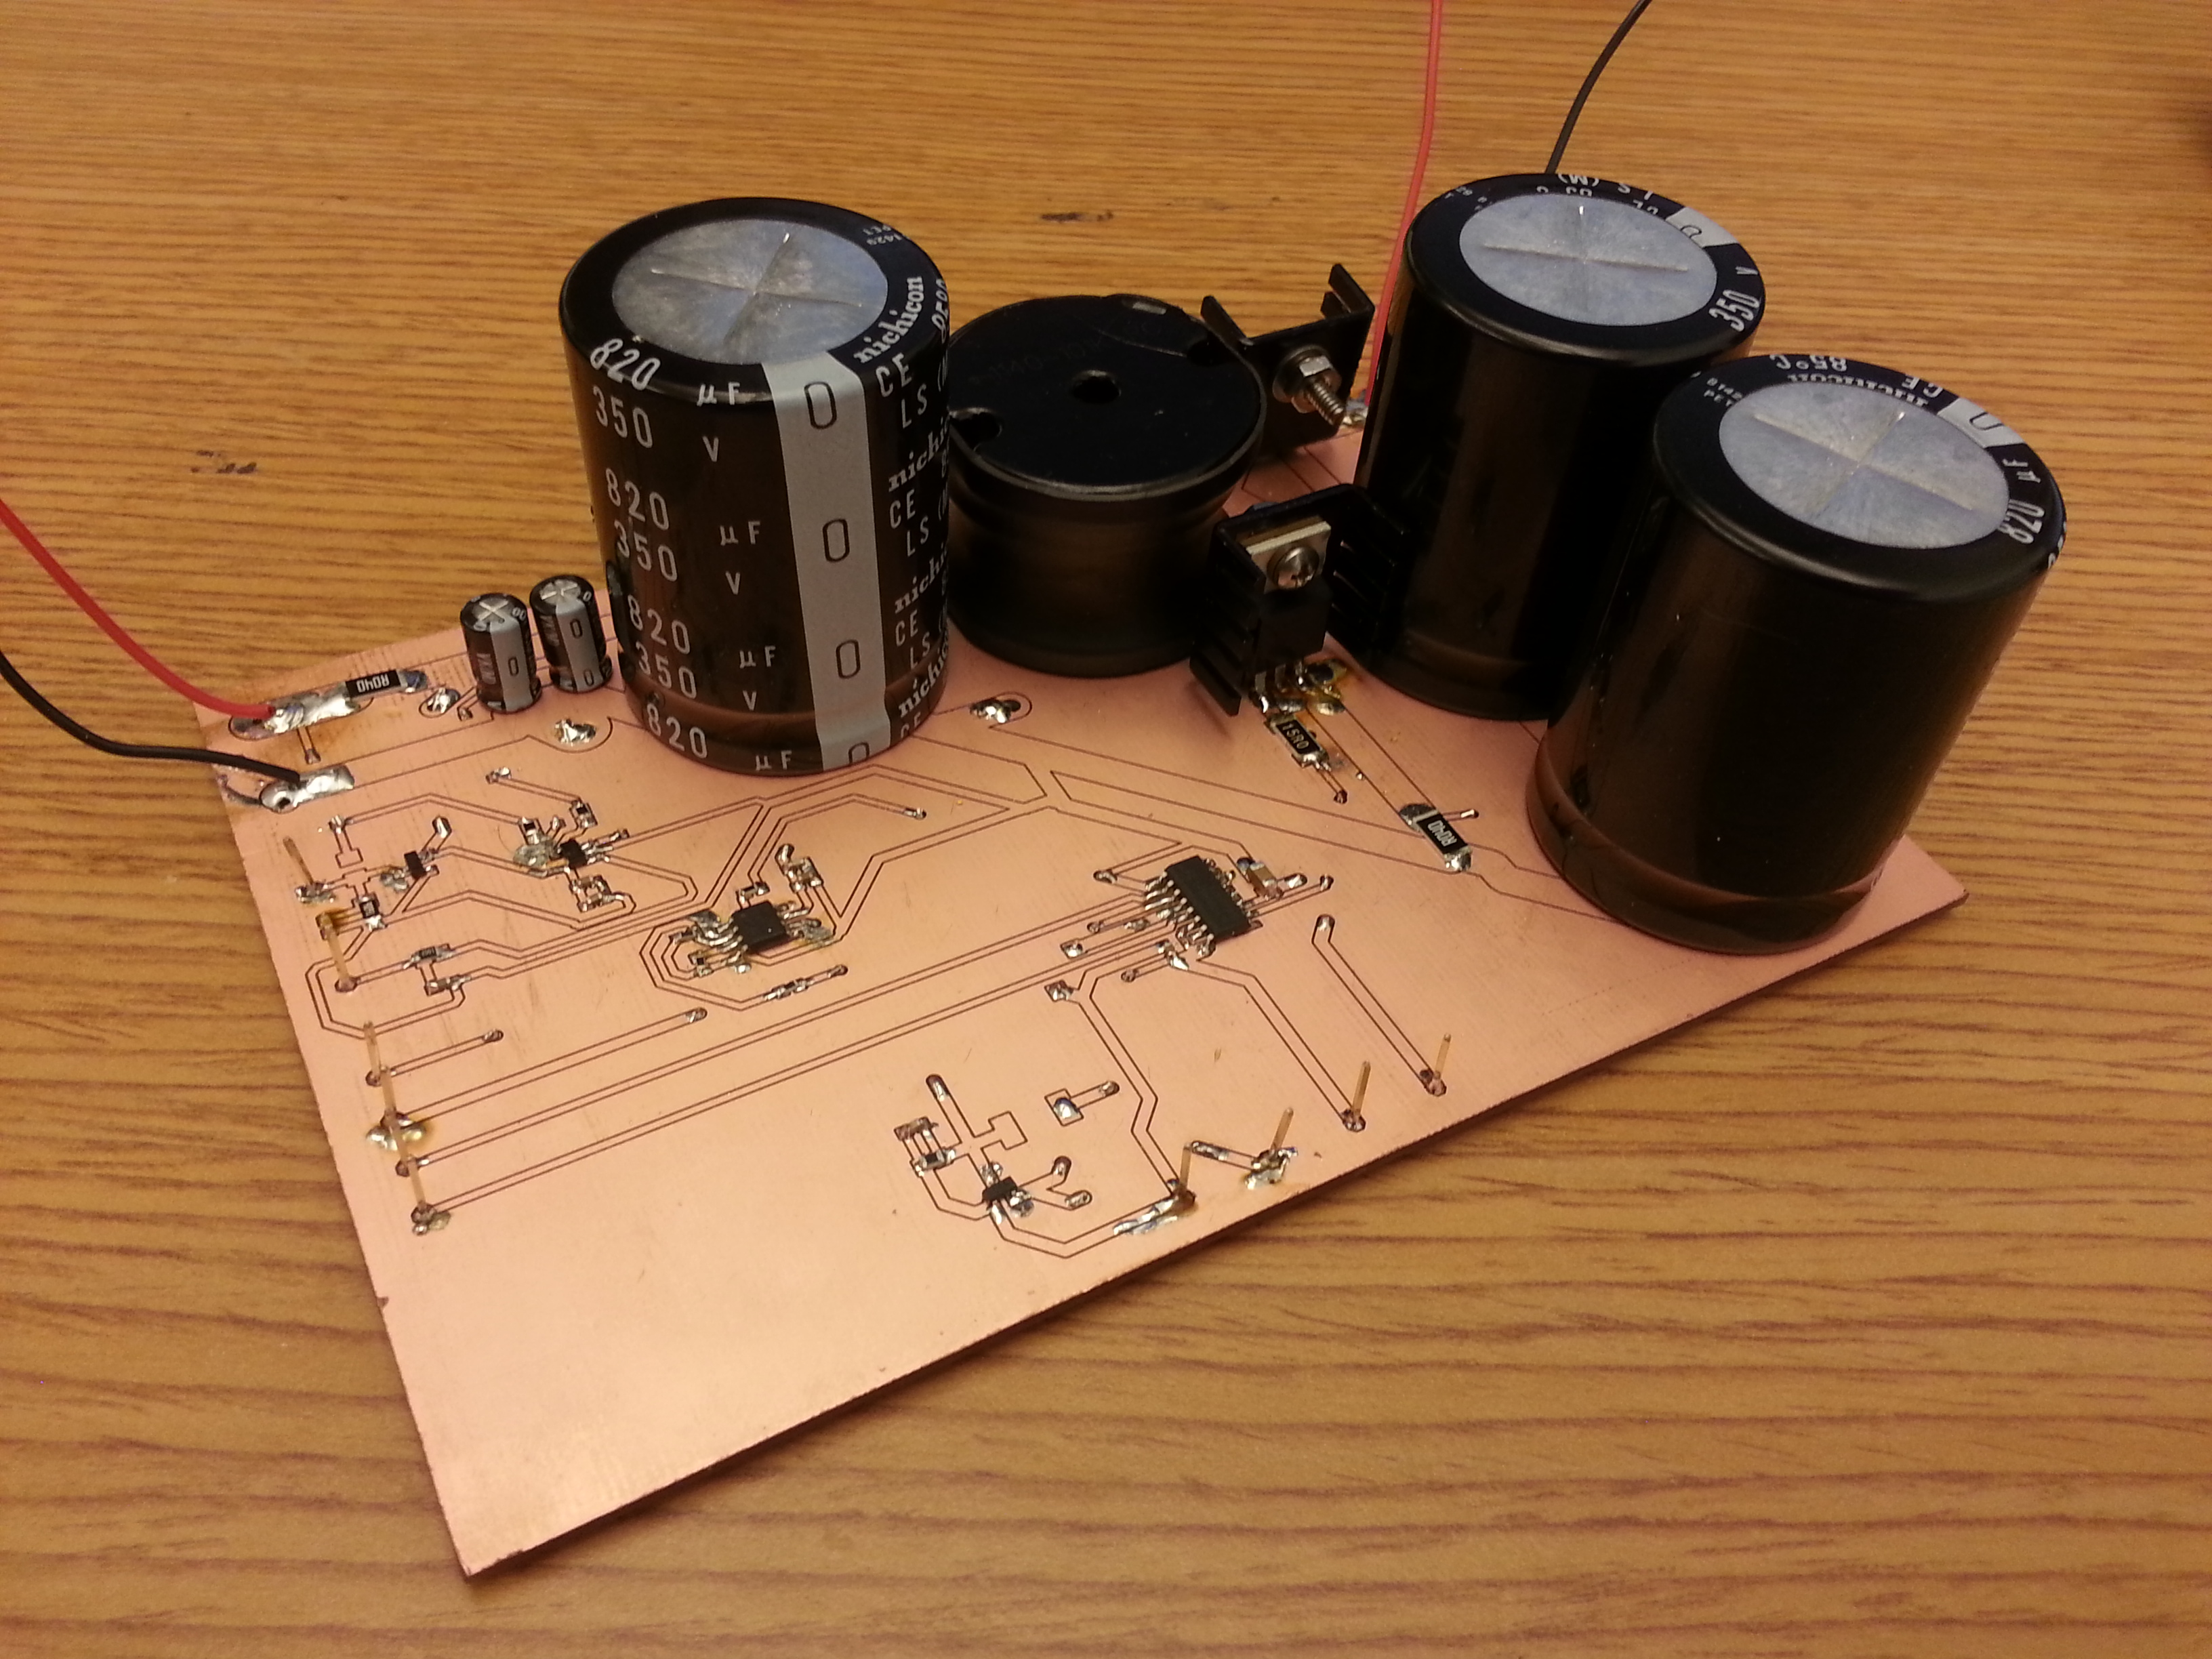
\includegraphics[width = 3.5in]{built_boost.jpg}
\caption{Assembled Boost Circuit}
\label{Built Boost}
\end{figure}

\subsection{H-Bridge}
Arguably, the lynch-pin of any inverter is the H-Bridge circuit. In order to generate a pseudo-sinusoid from a DC source, we must first have the means to switch this DC voltage on and off, and also to drive current bidirectionally. Thus, careful design of the H-Bridge circuit was a critical step in our development.

For a successful H-Bridge design, we needed to consider a number of factors including the speed of switching, deadband, transistor type, transistor gate drivers, thermal analysis, and careful layout due to the speed of the signals involved and the resultant EMI.

After some analysis of the algorithm, further discussed in Section (CITE ME!), we found that the speed of switching with the hybrid algorithm - unlike the switching speed of PWM algorithms which modulate over a fixed carrier frequency - was highly dependent on the width of the tracking band (@todo:Make sure that the tracking band is introduced in BG!). Consequently, there is also a dependence on the resolution of the ADC, and the frequency at which our interrupt is serviced. Through simulations in Matlab we were able to determine that the speed at which the algorithm caused the inverter to switch were well under 100kHz for a 'small-enough' tracking band. 

Because the switching speed is a function of width of the tracking band, sampling rate, and ADC resolution it is by no means a straightforward calculation to determine the frequency of switching. Contrast this to the PWM approach where this determination is trivial. In any case, because the switching speed was tunable by way of modifications to the with of the tracking band, it was decided that it was not necessary to go with more advanced FET technologies like Galium Nitride that are more than capable of switching in the MHz range under full load. 

Shoot through is another important consideration with the H-Bridge circuit, as the possibility of a nearly direct path from power to ground can exist as the circuit switches from outputting +Vdc to -Vdc. To prevent this, a mandatory off time just be implemented in hardware of software. We took the software approach, although the gate drivers we used also implement a minimal headband in hardware. In the configuration of the PWM driver in our micro controller code, a 20ns headband was implemented, based off of the 60MHz clock.

For the transistors in the H-Bridge, we decided on field effect transistors, (FETs), and in particular the CoolMOS\textsuperscript{TM}
variety built by Infineon. The IPP60 comes in a standard TO-220 package allowing for the use of standard heatsinks, has a Vds max of 650V - about three times what we would need - and a maximum continuous current of 31 Amps. Additionally, these FETs have a very low gate charge (low capacitance, smaller switching losses), low Rds on, and great slew rate. The fact that the drain to source resistance is low helps with our thermal budget, and also means higher efficiency overall. Because of the bipolar switching that the hybrid algorithm called for, we felt that it was wise to over specify our switches. Finally, the freewheeling diode found on many H-Bridge circuits was not needed here since the diode inherent to the construction of the FET was sufficient to handle any expected back currents in our load. 

\subsubsection{Switching Loss and Conduction Loss}
One of the primary factors in the overall efficiency of a modern switching power supply is the switching loss inherent to FET transistor technology, and also the conduction loss associated with Rds on, the resistance of the FET while it is conducting. Switching loss occurs whenever the FET changes state, and can be roughly understood as the net amount of charge it takes to drive the gate of the device. This amount of charge corresponds to a loss of current that could have gone to drive the load in question. This effect can be mitigated in some cases with parallel capacitance at the gate, using 'faster' FETs, and choice of the freewheeling diode\cite{switchingLoss}.

The heat sinks in our design are connected to the AC ground. Both the low-side and high-side transistors are insulated from the heat sink with thermal pads and insulating shoulder washers. According to the Transform application note we used as reference during our design, "For the high-side transistor, capacitance between the TO220 tab and the heat sink will add to switching loss, and so a thick and/or low permittivity insulator should be used."\cite{transphorm}

The gate drivers we chose, the SI823x family from Silicon Labs, have a built-in under voltage protection to prevent 'nuisance trips' and to add a good deal of noise margin. The gate drivers utilize a typical 'bootstrap' circuit to operate as both a high-side and low-side driver. 

Because of the relatively high speeds involved with the H-Bridge, careful layout was especially important here. Parasitic capacitance on gate and drain loops are a min cause of overshoot and ringing in the circuit, and thus the total enclosed area between the gate drive and the FETs was kept to the absolute minimum. In order to minimize inductance in the output current path, high current power and ground planes were utilized. Small ferrite beads were used between the gate drive output and the gates of the FETs to reduce ringing cause by coupling of the drain current to the gate drive loop- these were found to be more useful than small resistances which are sometimes used \cite{transphorm}. High voltage SMD ceramic bypass capacitors were placed directly underneath either side of the H-Bridge circuit to minimize the series inductance in the circuit. 
  
\subsection{RLC Filter}
In a typical PWM design, the driver behind the cutoff frequency of the output filter is the carrier frequency of the PWM signal. In most cases, this carrier frequency is invariant, and therefore allows for a relatively straightforward design parameter during the time where components are selected. Of course, THD is also a primary driver of part selection and valuation of the analog components.


In order to ensure that the vector fields on the power plane are such that the hybrid algorithm can ensure forward invariance, and that the solution of the system converges to the tracking band in finite time,  it is necessary that our design adhere to a set of constraints on the RLC filter described in \cite{ricardo}. 

Namely, our filter components must meet the following constraints: first, we must satisfy the condition that $LC\omega^2>1$ - this property ensures our vector fields are oriented correctly throughout the desired trajectory on the VI plane. Second, we have that the capacitor value must be determined by the output voltage amplitude and current amplitude by the relation:$\frac{I_l\omega}{V_c}$ where $I_l$ is the target output current, and $V_c$ is the target output voltage. From this final condition we observe that the value of the capacitance can be driven up by increasing the target current, decreasing the target voltage, or increasing the frequency of operation. 

Let's examine this mathematical condition through the lens of circuit analysis. By inspection, we note the similarity of this condition to the condition for resonance in a series RLC circuit - which is the subject of study in \cite{ricardo}. This condition is given by $\omega_0 = \frac{1}{\sqrt{LC}}$ Taking the square of both sides in the expression, find that $\omega_0^2LC=1$, and we see that the condition on the filter components given states that the resonant frequency of the circuit ought to be greater than unity. If we suppress the variable for capacitance in 
$LC\omega^2>1$ given the condition $C=\frac{I_l\omega}{V_c}$, we obtain:
\begin{equation}
\label{constraint}
L > \frac{V_c}{I_l\omega^2}
\end{equation}

The expression obtained in \ref{constraint} adds a considerable degree of inductance compared to that in a typical PWM inverter. it was considered initially that the quality factor, $Q$ might be at work in the conditions on the filter, but we find that the quality factor for the series RLC filter is given as $Q = \frac{1}{R}\sqrt{\frac{1}{LC}}$, and the analysis in \cite{ricardo} makes no mention of the damping term.

\subsection{AC Output Sensors}


\subsection{Microcontroller and USB-JTAG Interface}

\subsection{Complete Hardware System}
The final PCB layout utilized a four layer design with power and ground planes on the two middle layers. Multiple layers allowed for components to be placed closer together, and achieve a smaller overall form factor. Additionally, we were able to use polygon pours on the central power layers to boost current carrying capacity and aid in the dissipation of heat. Ground plane isolation was used to separate areas with switching power signal and digital logic.

Input and output connection points were placed around the perimeter of the board for easy interfacing with cables. Eagle PCB was utilized for this design and the board house Advanced Circuits was used for board fabrication. Parts were sourced from the Digikey. The top layer of the PCB is shown in Figure ~\ref{PCB top} and the bottom layer in Figure ~\ref{PCB bottom}. The completed circuit board is displayed in Figure ~\ref{hybrid_PCB}. 

%\begin{figure}
%\centering
%\includegraphics[width = 3.5in]{hybrid_pcb.jpg}
%\caption{PCB Complete}
%\label{PCB complete}
%\end{figure}

\begin{figure}
\centering
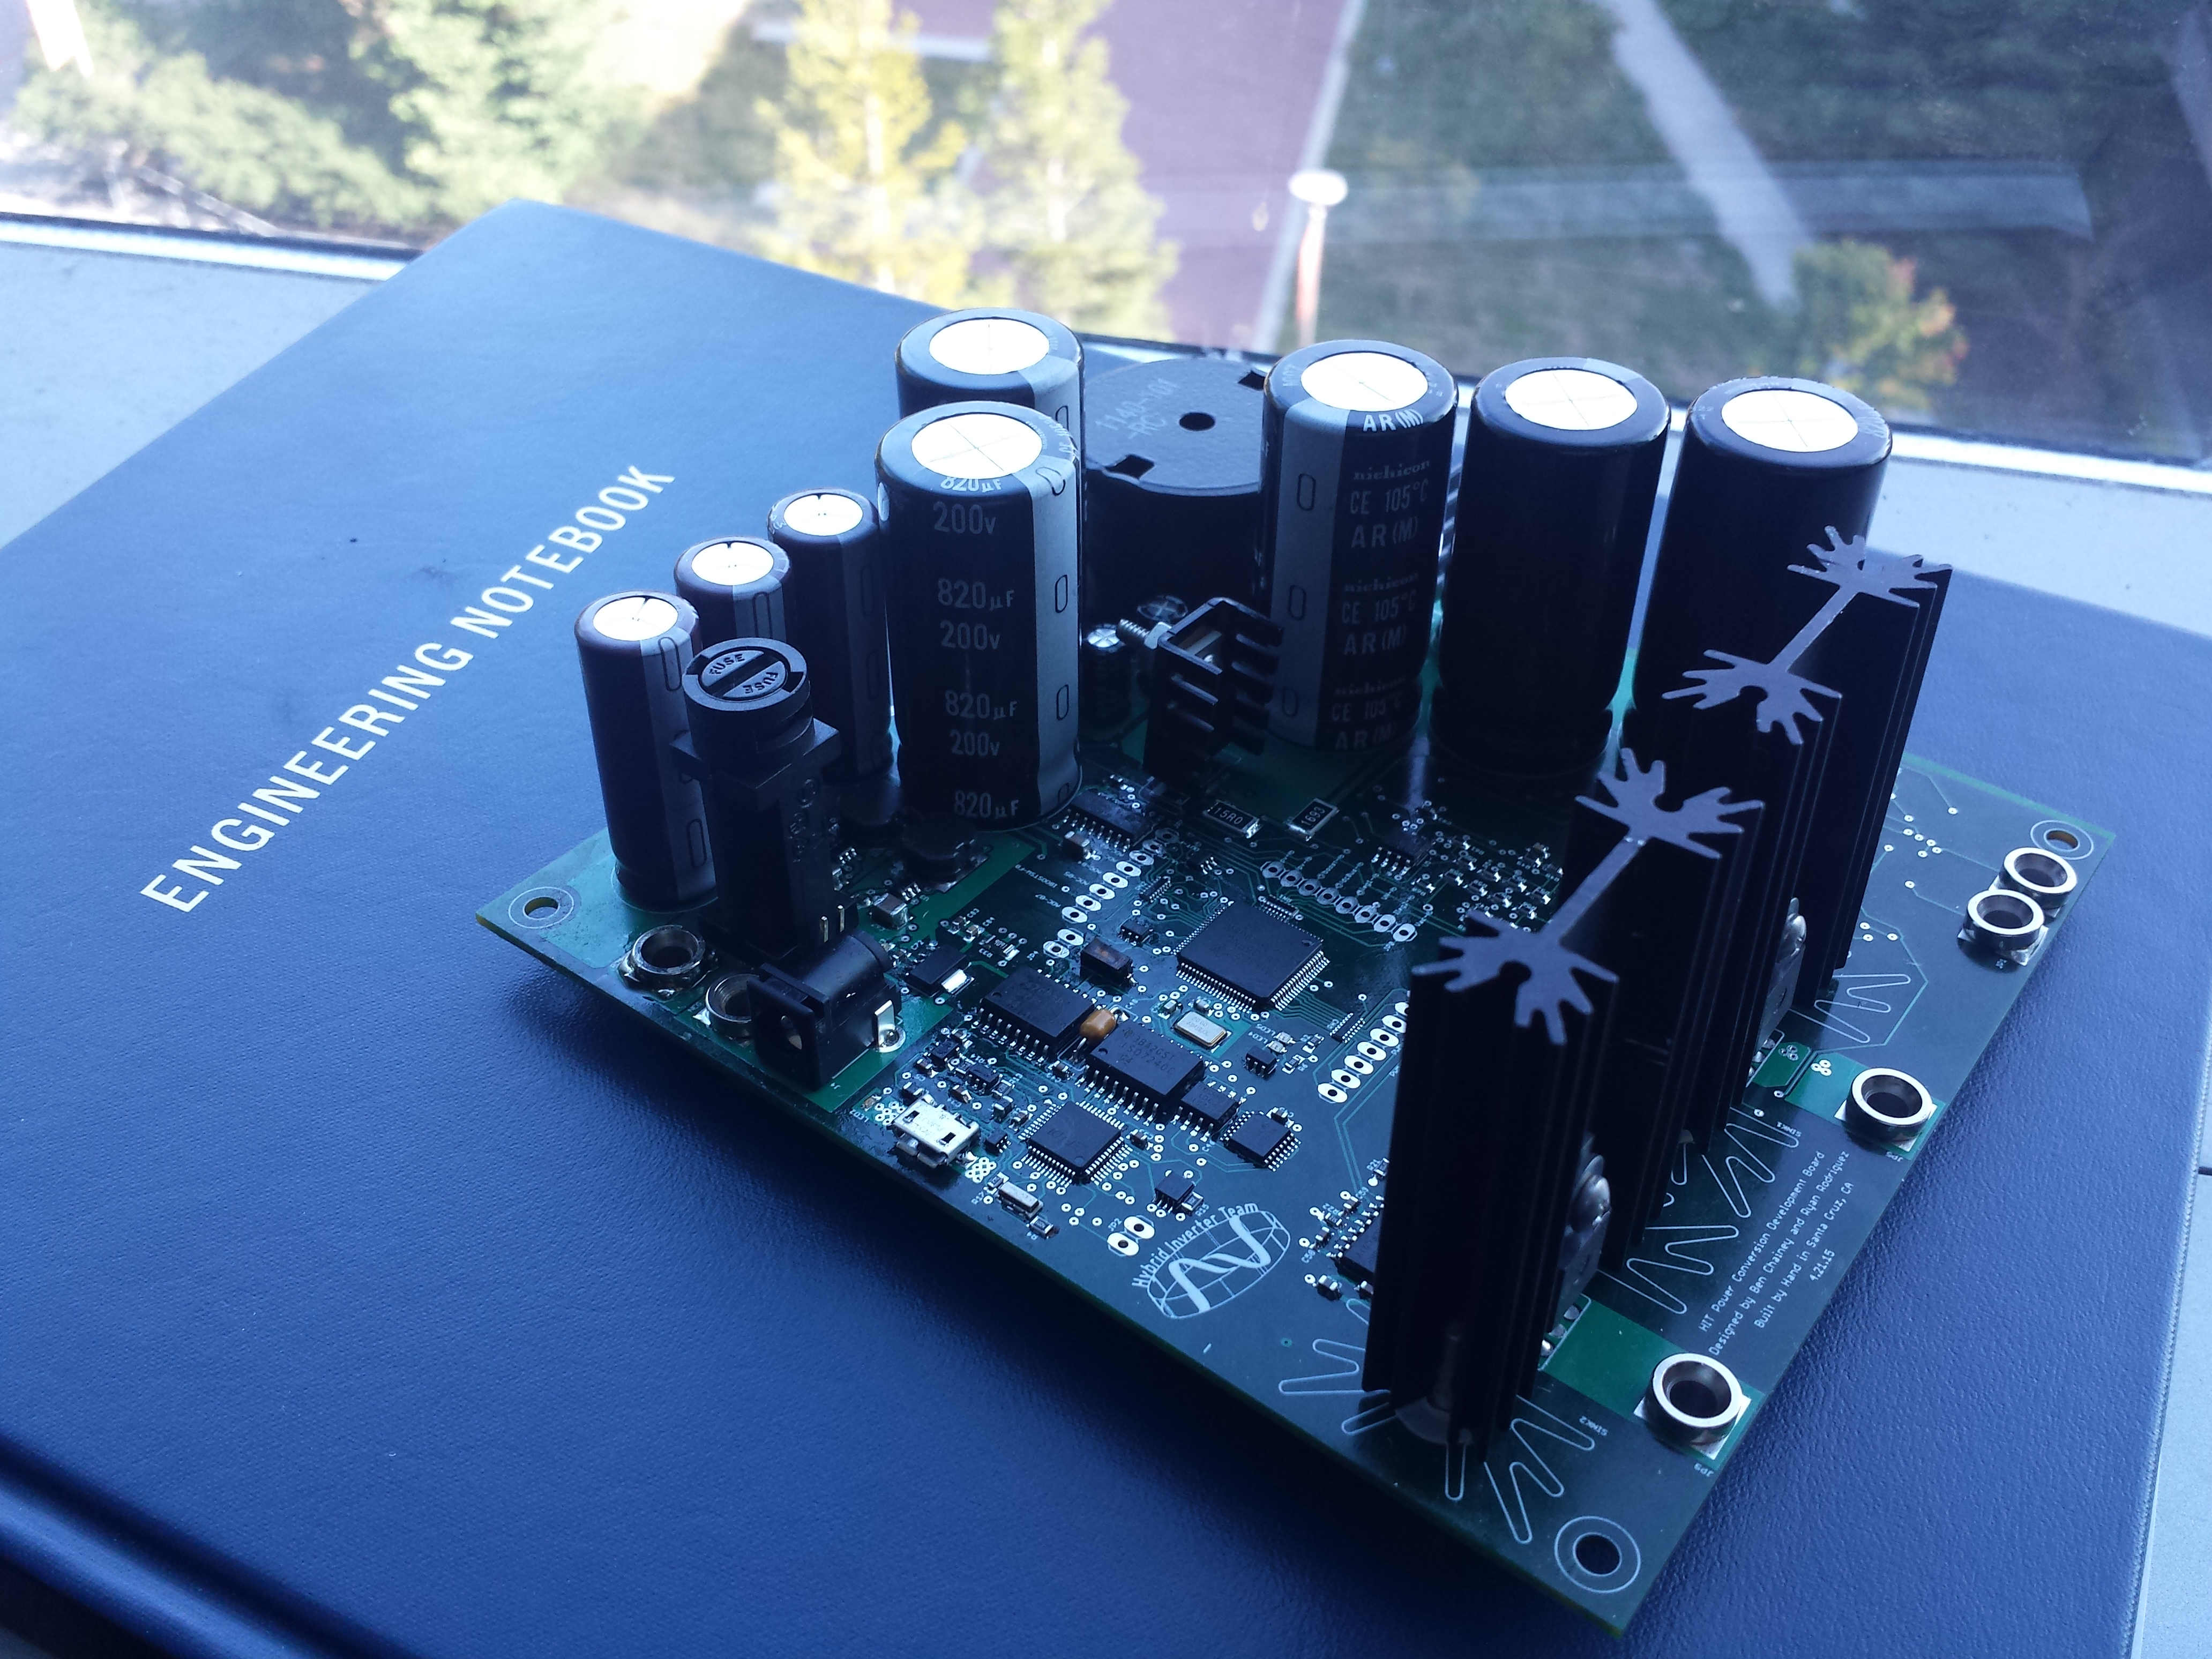
\includegraphics[width = 3.5in]{hitDevBoard}
\caption{The Hybrid Inverter Team's assembled PCB}
\label{The Hybrid Inverter Team's assembled PCB}
\end{figure}


The inverter sits in an enclosure mounted to the back of a solar panel to follow the microinverter topology. The output filter and transformer are constructed using turret board, and is also mounted on the panel mounting system. For testing in outdoor sunlight environments, a wooden stand for the solar panel and inverter system as shown in Figure~\ref{solar stand}.

\begin{figure}
\centering
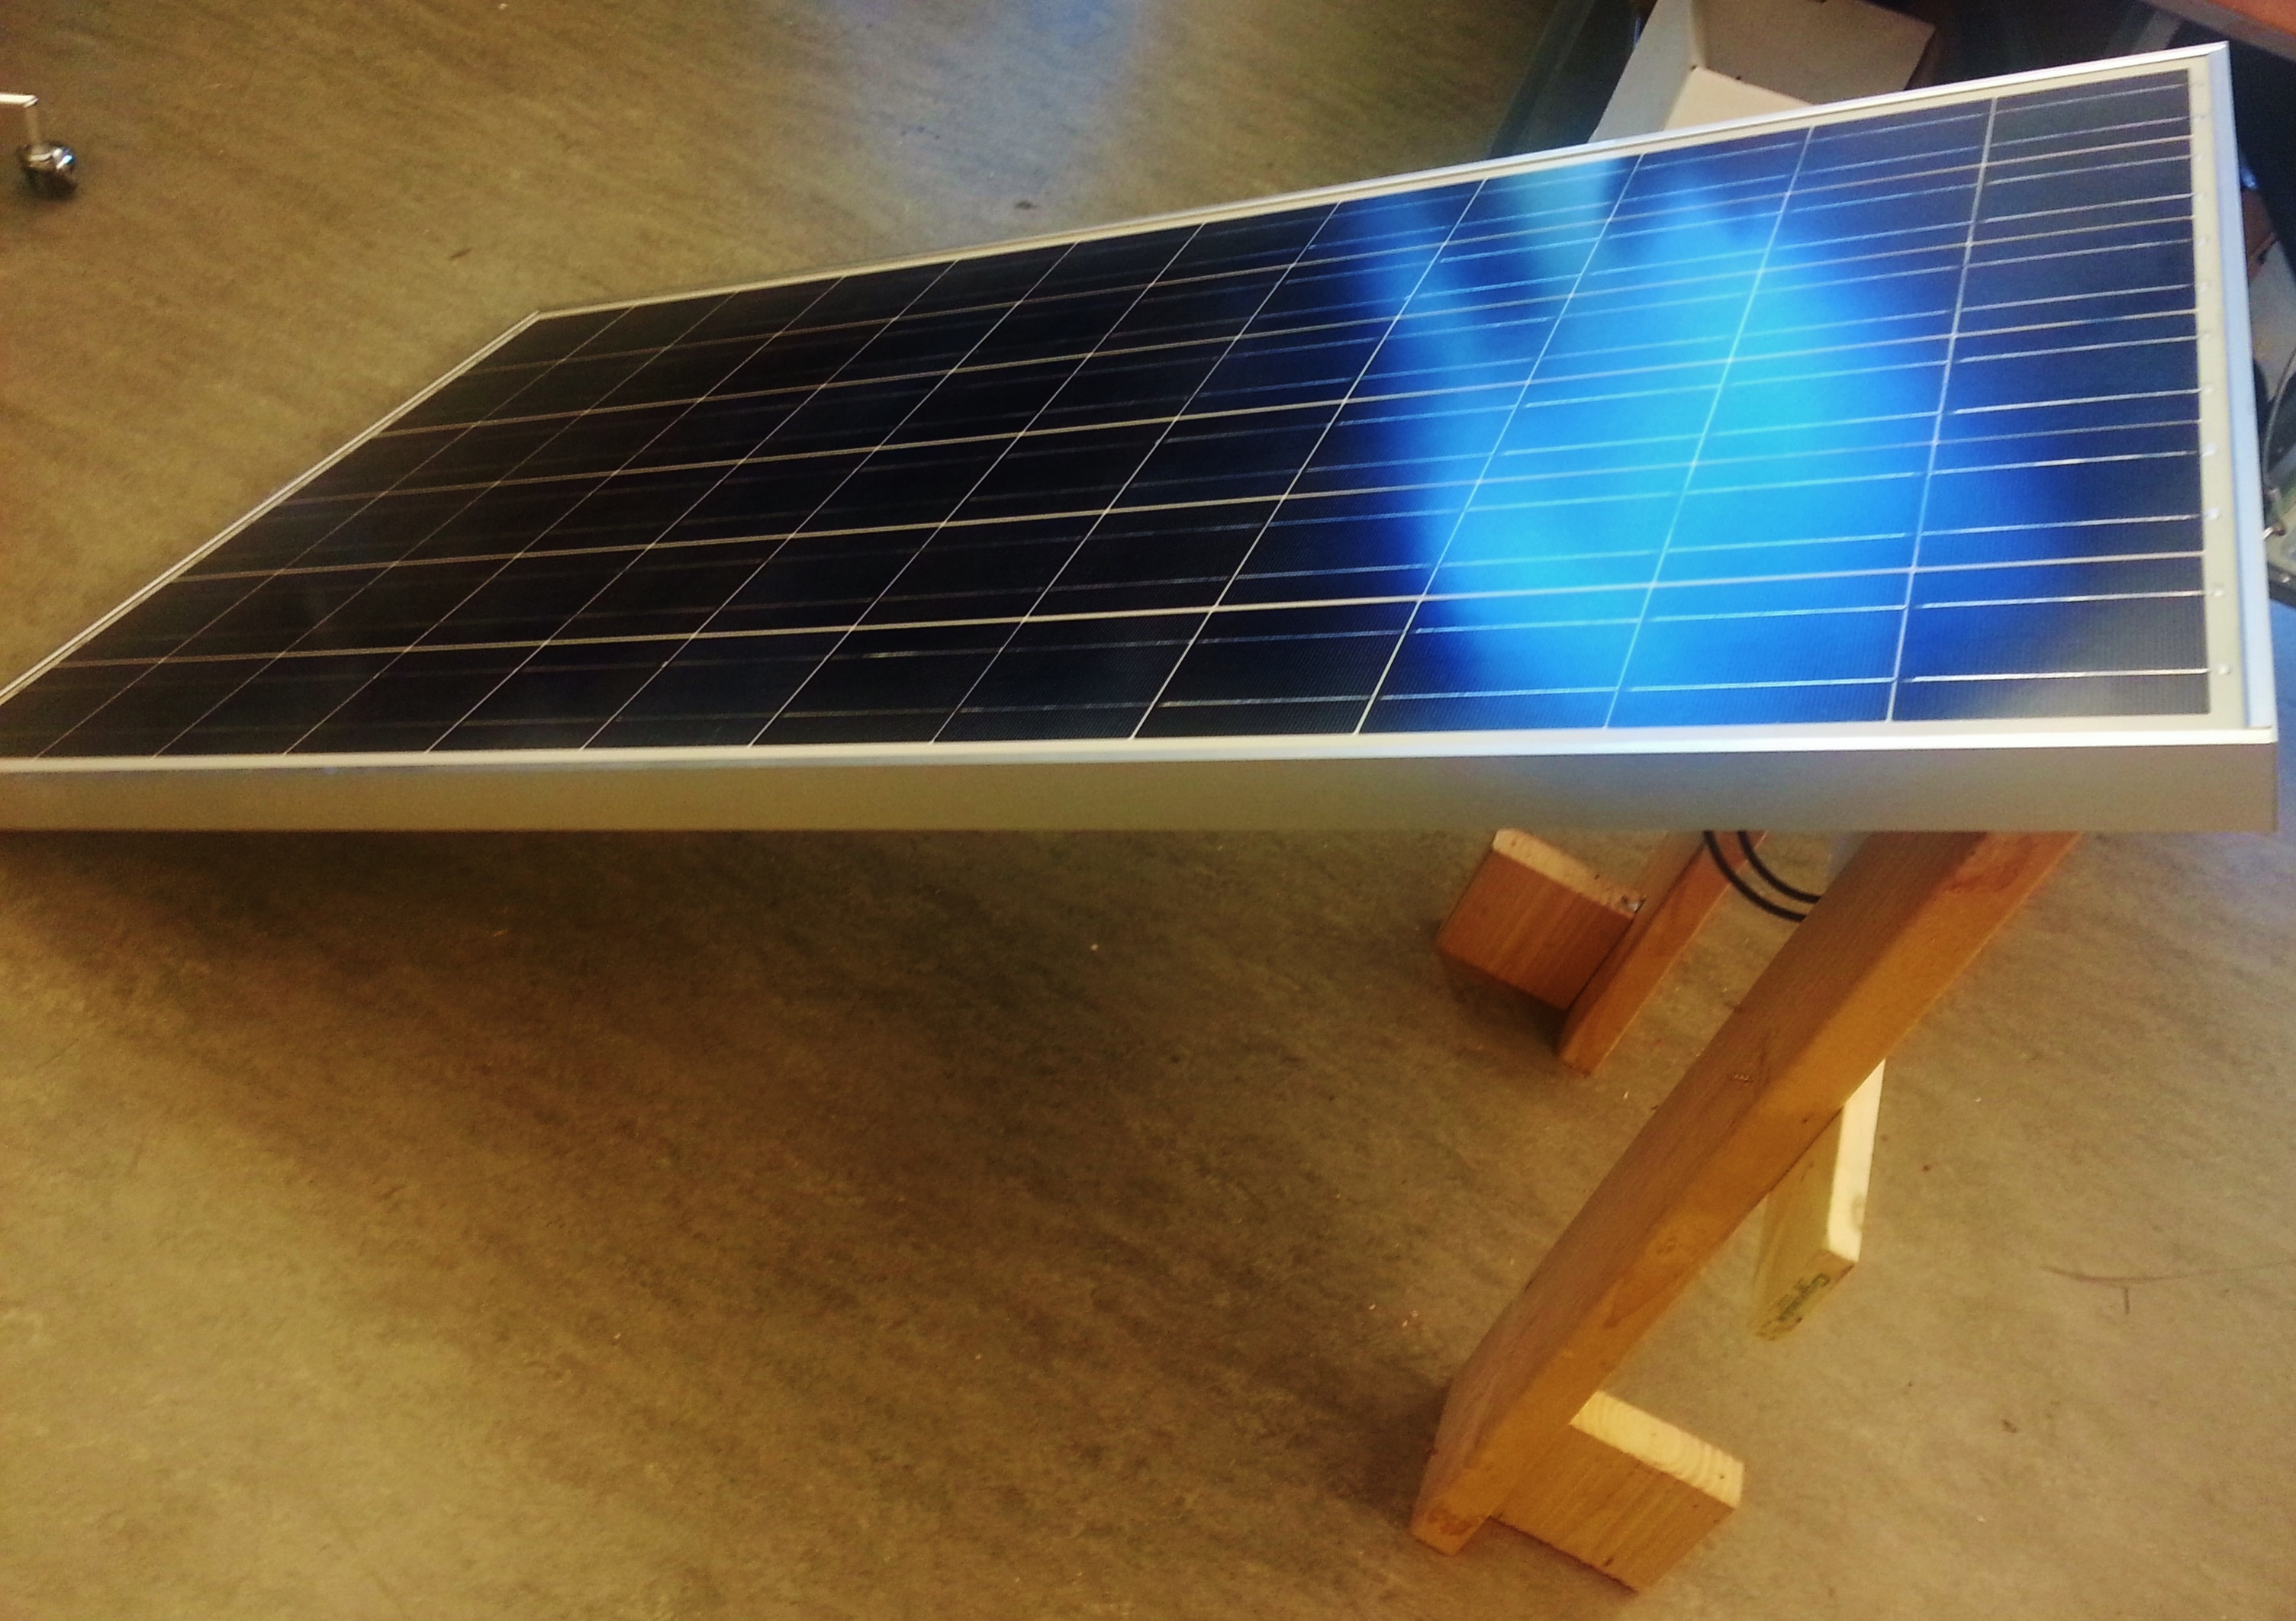
\includegraphics[width = 3.5in]{solar_stand.jpg}
\caption{Solar Panel Stand}
\label{solar stand}
\end{figure}





